\mysection{Résultats}
\mysubsection{Scripts}
En dessous les résultats provenus des scripts crées dans la troisième partie du projet. 

\begin{itemize}
\item $\mathbf{gain\_calc-load2bus}$\\
\\
\begin{table}[H]\tiny
	\captionsetup{justification=centering,margin=2cm}
	\caption{Matrice des Gain entre Puissance Réactive des charges et la tension des Bus ( Valeurs numériques )}
	\centering
	\resizebox{\textwidth}{!}{\begin{tabular}{ccccccccccccccccc}
			%	1&2&3&4&5&6&7&8&9&10&11&12&13&14&15&16\\
			0e+0& -9.0e-5& -1.1e-4& -1.1e-4& -1.1e-4& -1.1e-4& -1.1e-4& -1.1e-4& -1.1e-4& -1.1e-4& -1.1e-4& -1.1e-4& -1.1e-4& -1.1e-4& -1.1e-4& -1.1e-4\\
			0e+0& -8.9e-5& -1.1e-4& -1.3e-4& -1.3e-4& -1.3e-4& -1.3e-4& -1.3e-4& -1.3e-4& -1.3e-4& -1.3e-4& -1.3e-4& -1.3e-4& -1.3e-4& -1.3e-4& -1.3e-4\\
			0e+0& -9.1e-5& -1.1e-4& -1.3e-4& -1.8e-4& -1.8e-4& -1.8e-4& -1.8e-4& -1.8e-4& -1.8e-4& -1.8e-4& -1.8e-4& -1.8e-4& -1.8e-4& -1.8e-4& -1.8e-4\\
			0e+0& -1.2e-4& -1.5e-4& -1.8e-4& -2.5e-4& -3.5e-4& -4.2e-4& -4.2e-4& -4.2e-4& -4.2e-4& -4.2e-4& -3.4e-4& -3.4e-4& -3.4e-4& -3.4e-4& -3.4e-4\\
			0e+0& -9.4e-5& -1.2e-4& -1.4e-4& -1.9e-4& -2.7e-4& -3.3e-4& -3.9e-4& -3.9e-4& -3.9e-4& -3.9e-4& -2.6e-4& -2.6e-4& -2.6e-4& -2.6e-4& -2.6e-4\\
			0e+0& -9.5e-5& -1.2e-4& -1.4e-4& -1.9e-4& -2.7e-4& -3.3e-4& -4.0e-4& -4.3e-4& -4.3e-4& -4.3e-4& -2.7e-4& -2.6e-4& -2.6e-4& -2.7e-4& -2.7e-4\\
			0e+0& -9.3e-5& -1.2e-4& -1.4e-4& -1.9e-4& -2.6e-4& -3.2e-4& -3.8e-4& -4.2e-4& -4.5e-4& -4.5e-4& -2.6e-4& -2.6e-4& -2.6e-4& -2.6e-4& -2.6e-4\\
			0e+0& 0e+0& 0e+0& 0e+0& 0e+0& 0e+0& 0e+0& 0e+0& 0e+0& 0e+0& 0e+0& 0e+0& 0e+0& 0e+0& 0e+0& 0e+0\\
			0e+0& 0e+0& 0e+0& 0e+0& 0e+0& 0e+0& 0e+0& 0e+0& 0e+0& 0e+0& 0e+0& 0e+0& 0e+0& 0e+0& 0e+0& 0e+0\\
			0e+0& -9.7e-5& -1.2e-4& -1.4e-4& -2.0e-4& -2.7e-4& -3.4e-4& -4.0e-4& -4.4e-4& -4.8e-4& -5.2e-4& -2.7e-4& -2.7e-4& -2.7e-4& -2.7e-4& -2.7e-4\\
			0e+0& -9.5e-5& -1.2e-4& -1.4e-4& -1.9e-4& -2.7e-4& -2.7e-4& -2.7e-4& -2.7e-4& -2.7e-4& -2.7e-4& -2.8e-4& -2.8e-4& -2.8e-4& -2.8e-4& -2.8e-4\\
			0e+0& -9.1e-5& -1.1e-4& -1.3e-4& -1.9e-4& -2.6e-4& -2.6e-4& -2.6e-4& -2.6e-4& -2.6e-4& -2.6e-4& -2.7e-4& -2.8e-4& -2.8e-4& -2.9e-4& -2.9e-4\\
			0e+0& -9.5e-5& -1.2e-4& -1.4e-4& -1.9e-4& -2.7e-4& -2.7e-4& -2.7e-4& -2.7e-4& -2.7e-4& -2.7e-4& -2.8e-4& -3.0e-4& -3.1e-4& -3.1e-4& -3.1e-4\\
			0e+0& -9.3e-5& -1.2e-4& -1.4e-4& -1.9e-4& -2.6e-4& -2.6e-4& -2.7e-4& -2.7e-4& -2.7e-4& -2.7e-4& -2.8e-4& -2.9e-4& -3.1e-4& -3.2e-4& -3.2e-4\\
			0e+0& 0e+0& 0e+0& 0e+0& 0e+0& 0e+0& 0e+0& 0e+0& 0e+0& 0e+0& 0e+0& 0e+0& 0e+0& 0e+0& 0e+0& 0e+0\\
			0e+0& -9.2e-5& -1.2e-4& -1.4e-4& -1.9e-4& -2.6e-4& -2.6e-4& -2.6e-4& -2.6e-4& -2.6e-4& -2.6e-4& -2.8e-4& -2.9e-4& -3.0e-4& -3.2e-4& -3.4e-4
			\\
	\end{tabular}}
\end{table} 
\item $\mathbf{gain\_calc-generator2bus}$\\
\begin{itemize}
	
\item $\mathbf{gain\_calc-generator2bus-test\_1-7am}$\\
\\Ce script calcule le gain entre la puissance réactive des générateurs et la tension des bus aux lesquels ils sont connectés, avec les valeurs de charges de 7 heures et en faisant la puissance réactive des générateurs diminuer en 20\%.
\begin{table}[H]
	\captionsetup{justification=centering,margin=2cm}
	\caption{Matrice des Gain entre Puissance Réactive des générateurs et la tension des Bus ( Valeurs numériques )}
	\centering
	\begin{tabular}{ccc}
		1.7e-4&1.7e-4&1.7e-4\\
		1.7e-4&2.5e-4&2.7e-4\\
		1.7e-4&3.1e-4&2.4e-4\\
	\end{tabular}
\end{table}

\item $\mathbf{gain\_calc-generator2bus-test\_1-1pm}$\\
\\
Ce script calcule le gain entre la puissance réactive des générateurs et la tension des bus aux lesquels ils sont connectés, avec les valeurs de charges de 13 heures et en faisant la puissance réactive des générateurs diminuer en 20\%.

\begin{table}[H]
	\captionsetup{justification=centering,margin=2cm}
	\caption{Matrice des Gain entre Puissance Réactive des générateurs et la tension des Bus ( Valeurs numériques )}
	\centering
	\begin{tabular}{ccc}
		1.7e-4&1.7e-4&1.6e-4\\
		1.7e-4&2.4e-4&2.7e-4\\
		1.7e-4&3.0e-4&2.4e-4\\
	\end{tabular}
	
\end{table}

\item $\mathbf{gain\_calc-generator2bus-test\_2}$\\
\\Ce script calcule le gain entre la puissance réactive des générateurs et la tension des bus aux lesquels ils sont connectés, avec les valeurs de charges de 13 heures et en faisant la puissance réactive des générateurs augmenter en 20\%.

\begin{table}[H]
	\captionsetup{justification=centering,margin=2cm}
	\caption{Matrice des Gain entre Puissance Réactive des générateurs et la tension des Bus ( Valeurs numériques )}
	\centering
	\begin{tabular}{ccc}
		
		1.8e-4&1.8e-4&1.7e-4\\
		
		1.8e-4&2.5e-4&2.8e-4\\
		
		1.8e-4&3.1e-4&2.5e-4\\
	\end{tabular}
\end{table}

\end{itemize}
\item $\mathbf{teste\_simul}$\\
\\Ce script crée un événement des changement de valeur de puissance active de la charge C 2-29 MT ind en augmentant sa valeur en 100\% par un période de temps et après prend les valeurs de puissance active et réactive des cette même charge et la tension des bus N21 N23 et N29 ( où les générateurs sont connectés ) pendant le temps de la simulation et en exportant en un fichier $ \verb|.csv| $ pour faire des graphiques, figures \ref{fig:Puissance_Active_et_Reactive_de_la_Charge_C2_29_MT} et \ref{fig:Tension_des_Bus_N21_N23_et_N29}.\\
\begin{minipage}{.5\textwidth}
	\begin{figure}[H]
		\begin{center}
			\captionsetup{justification=centering,margin=.5cm}	
			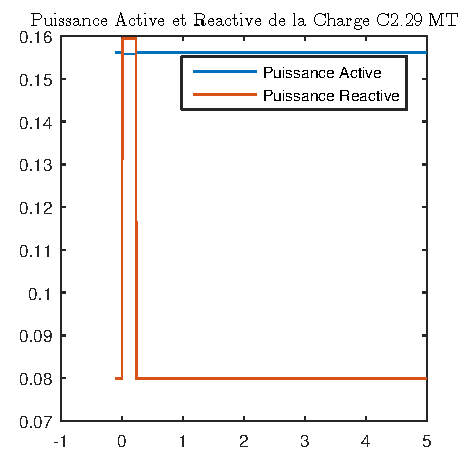
\includegraphics[width=\textwidth]{Resultats/Puissance_Active_et_Reactive_de_la_Charge_C2_29_MT.pdf}
			\caption{Puissance Active et Réactive \\de la Charge C2 29 MT}
			\label{fig:Puissance_Active_et_Reactive_de_la_Charge_C2_29_MT}
		\end{center}
	\end{figure}
\end{minipage}

\begin{minipage}{.5\textwidth}
	\begin{figure}[H]
		\begin{center}
			\captionsetup{justification=centering,margin=.5cm}	
			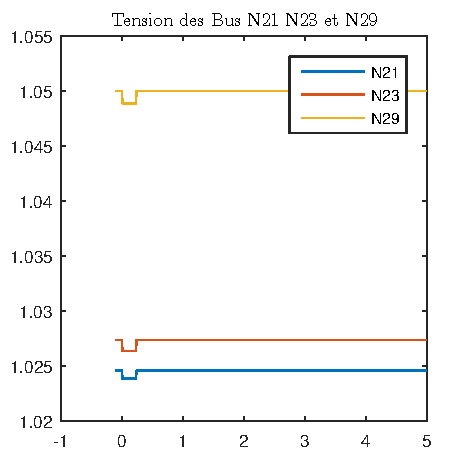
\includegraphics[width=\textwidth]{Resultats/Tension_des_Bus_N21_N23_et_N29.pdf}
			\caption{Tension des Bus N21 N23 et N29 en p.u.}
			\label{fig:Tension_des_Bus_N21_N23_et_N29}
		\end{center}
	\end{figure}
\end{minipage}
\end{itemize}